\section{La planta (provista)}

\begin{frame}{Modelo dinámico híbrido de la planta}
  La cátedra entrega el modelo completo. Es \textbf{híbrido}: combina dinámicas continuas con
  cambios discretos de estado.
  \begin{columns}[T]
    \begin{column}{0.5\textwidth}
      \begin{block}{Variables continuas (\textit{flow})}
        \begin{itemize}
          \item Posición/velocidad de carro $x_t,v_t$ e izaje $y_h,v_h$.
          \item Ángulo de balanceo $\theta_l$, tensión de cable $F_{hw}$.
          \item Torques, fuerzas de contacto.
        \end{itemize}
      \end{block}
    \end{column}
    \begin{column}{0.5\textwidth}
      \begin{block}{Estados discretos (\textit{jump})}
        \begin{itemize}
          \item Twistlocks \sig{TLK}: abierto/cerrado.
          \item Contacto: suspendido/apoyado.
          \item Cable: tenso/flojo.
          \item Frenos NC \sig{$BRK$}: abierto/cerrado.
        \end{itemize}
      \end{block}
    \end{column}
  \end{columns}
  \vspace{0.3cm}
  \centering
  \footnotesize Carro e izaje acoplados por la carga pendular; interacción con el perfil de
  obstáculos del entorno.
\end{frame}

\begin{frame}{Implementación de la planta en Simulink}
  \begin{columns}[T]
    \begin{column}{0.62\textwidth}
      \centering
      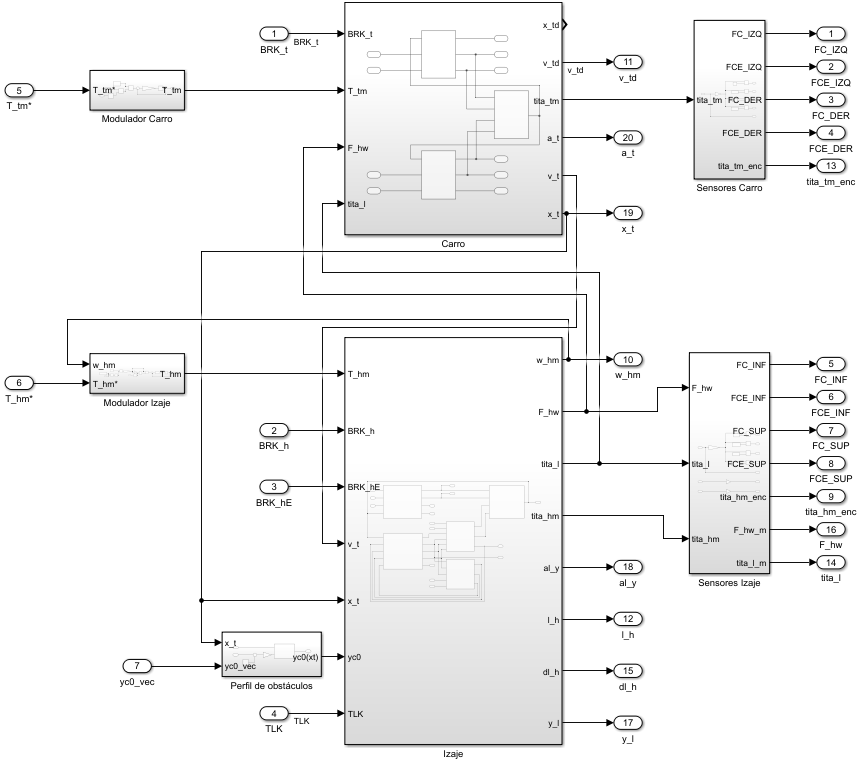
\includegraphics[width=\linewidth]{modelo_planta.png}
    \end{column}
    \begin{column}{0.38\textwidth}
      \footnotesize
      \begin{block}{Parámetros (dados)}
        \begin{tabular}{ll}
          $M_t$ & $30\,000$ kg \\
          $M_s$ & $15\,000$ kg \\
          $M_{c\max}$ & $50\,000$ kg \\
          $i_t / i_h$ & $30 / 22$ \\
          $v_{t\max}$ & $4$ m/s \\
          $v_{h}$ & $1.5$--$3$ m/s \\
        \end{tabular}
      \end{block}
      Sensores: encoders, fines de carrera, celda de carga, ángulo de spreader, LIDAR.
    \end{column}
  \end{columns}
\end{frame}

\begin{frame}{Subsistema del carro: visión general}
  \begin{block}{Función del sistema}
    Traslación horizontal del carro mediante un \textbf{motor} que acciona un \textbf{tambor},
    el cual tira del carro a través de cables de acero.
  \end{block}

  \begin{block}{Modelo: sistema electromecánico de 2 masas}
    \begin{itemize}
      \item \textbf{Masa rotacional}: inercia del accionamiento (motor + tambor + reductor).
      \item \textbf{Masa traslacional}: el carro $M_t$ sobre los rieles.
      \item Acopladas por un \textbf{cable elástico} (resorte-amortiguador).
    \end{itemize}
  \end{block}

  \begin{alertblock}{Hipótesis}
    Transmisión rígida y \textbf{1 cable equivalente} de carro, siempre tensado, con elasticidad
    longitudinal amortiguada.
  \end{alertblock}
\end{frame}

\begin{frame}{Dinámica del carro (2.\textsuperscript{a} ley de Newton)}
  \begin{block}{Movimiento horizontal del carro}
    \[
    M_t \, \frac{dv_t(t)}{dt} = F_{tw}(t) - b_t \, v_t(t) + 2 F_{hw}(t)\sin\theta_l(t)
    \]
  \end{block}

  \vspace{-0.1cm}
  \begin{block}{Términos}
    \begin{itemize}
      \item $F_{tw}(t)$: fuerza de tracción del cable del carro.
      \item $b_t \, v_t(t)$: fricción viscosa sobre los rieles.
      \item $2 F_{hw}(t)\sin\theta_l(t)$: fuerza horizontal por el balanceo de la carga.
    \end{itemize}
    Valores: $M_t = 30\,000$ kg \quad ; \quad $b_t = 90$ Ns/m.
  \end{block}

  \begin{alertblock}{Acoplamiento con el izaje}
    El término $2 F_{hw}\sin\theta_l$ es la \textbf{perturbación del balanceo}: conecta la
    dinámica del carro con la de la carga suspendida.
  \end{alertblock}
\end{frame}

\begin{frame}{Acoplamiento elástico del cable}
  \begin{block}{Modelo resorte-amortiguador}
    El cable transmite la fuerza entre el tambor y el carro:
    \[
    F_{tw}(t) = K_{tw}\,\big(x_{td}(t) - x_t(t)\big) + b_{tw}\,\big(v_{td}(t) - v_t(t)\big)
    \]
  \end{block}

  \begin{block}{Parámetros y variables}
    \begin{itemize}
      \item $K_{tw} = 480 \times 10^3$ N/m \quad (rigidez del cable).
      \item $b_{tw} = 3 \times 10^3$ Ns/m \quad (amortiguamiento).
      \item $x_{td},\,v_{td}$: posición y velocidad lineal \textbf{equivalente del tambor}
            (en su superficie).
    \end{itemize}
  \end{block}

  \begin{alertblock}{Interpretación}
    La fuerza depende de la \textbf{diferencia} tambor--carro: el cable se estira y empuja/tira
    según el desfasaje entre ambos.
  \end{alertblock}
\end{frame}

\begin{frame}{Dinámica del accionamiento: dos ejes}
  \begin{columns}[T]
    \begin{column}{0.4\textwidth}
      \textbf{Eje lento (tambor)}
      \[ J_{td}\,\dot\omega_{td}(t) = T_{td}(t) - b_{td}\,\omega_{td}(t) - T_{tdl}(t) \]
      \begin{itemize}
        \item $J_{td} = 1200$ kgm²
        \item $b_{td} = 1.8$ Nms/rad
        \item $r_{td} = 0.5$ m
        \item $T_{tdl}(t) = F_{tw}(t)\,r_{td}$ (carga del cable)
      \end{itemize}
    \end{column}
    \begin{column}{0.6\textwidth}
      \textbf{Eje rápido (motor)}
      \[ J_{tm+tb}\,\dot\omega_{tm}(t) = T_{tm}(t) + T_{tb}(t,\sig{BRK_t}) - b_{tm}\,\omega_{tm}(t)- T_{tml}(t) \]
      \begin{itemize}
        \item $J_{tm+tb} = 7$ kgm²
        \item $b_{tm} = 6$ Nms/rad
        \item $T_{tm}(t)$: torque del motor
        \item $T_{tb}(t,\sig{BRK_t})$: torque del freno
      \end{itemize}
    \end{column}
  \end{columns}

  \vspace{0.2cm}
  \begin{alertblock}{Unión de los ejes}
    Reductor de relación $i_t = 30$: $\;\omega_{td}\,i_t = \omega_{tm}\;$ y $\;T_{td} = i_t\,T_{tml}$.
  \end{alertblock}
\end{frame}

\begin{frame}{Freno mecánico (Normal Cerrado)}
  \begin{block}{Torque de frenado --- depende de \sig{$BRK_t$}}
    \[
    T_{tb}(\sig{BRK_t}) =
    \begin{cases}
      0 & \sig{BRK_t}=1 \;(\text{abierto}) \\[4pt]
      -T_{tb\max}\tanh(b_{tb}\,\omega_{tm}) & \sig{BRK_t}=0 \;(\text{cerrado})
    \end{cases}
    \]
    \begin{columns}[c]
      \begin{column}{0.42\textwidth}
        \begin{itemize}
          \item $T_{tb\max} = 5 \times 10^3$ Nm
          \item $b_{tb} = 5 \times 10^6$ Nms/rad
        \end{itemize}
      \end{column}
      \begin{column}{0.48\textwidth}
        \centering
        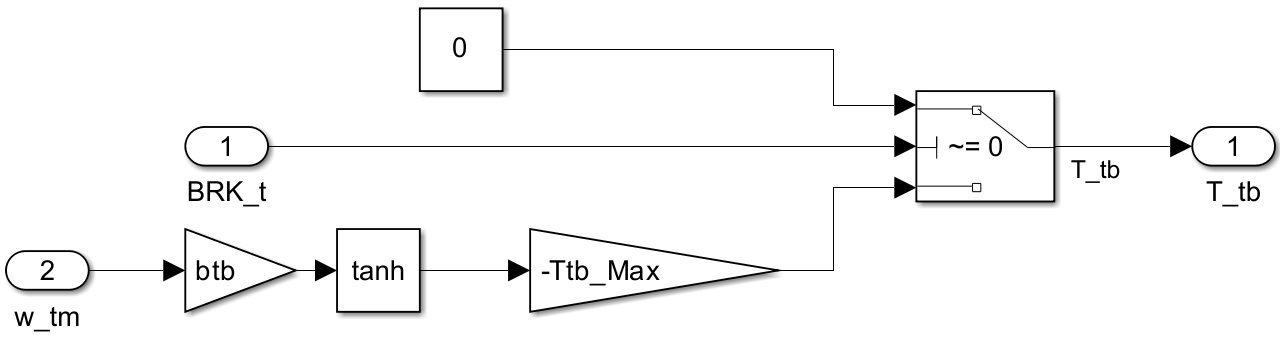
\includegraphics[width=\linewidth]{freno_carro.png}
      \end{column}
    \end{columns}
  \end{block}

  \begin{alertblock}{Por qué $\tanh$}
    Función continua y abrupta: frena fuerte pero evita la \textbf{discontinuidad numérica}
    del signo en la simulación.
  \end{alertblock}
\end{frame}

\begin{frame}{Modelo equivalente referido al motor}
  \begin{block}{Reducción a un solo eje}
    Se refiere la dinámica del tambor al eje del motor usando $i_t = 30$, agrupando inercias y
    fricciones:
  \end{block}

  \vspace{-0.2cm}
  \[
  J_{t,eq} = J_{tm+tb} + \frac{J_{td}}{i_t^2} = 7 + \frac{1200}{30^2} \approx 8.33 \text{ kgm}^2
  \]
  \vspace{-0.2cm}
  \[
  b_{t,eq} = b_{tm} + \frac{b_{td}}{i_t^2} = 6 + \frac{1.8}{30^2} \approx 6.002 \text{ Nms/rad}
  \]

  \begin{alertblock}{Resultado}
    Ecuación de estado única para todo el accionamiento del carro:
    \[
    \frac{d\omega_{tm}}{dt}(t) = \frac{1}{J_{t,eq}}\left[T_{tm}(t) + T_{tb}(t,\sig{BRK_t}) - b_{t,eq}\,\omega_{tm}(t)
      - \frac{r_{td}}{i_t}F_{tw}(t)\right]
    \]
  \end{alertblock}
\end{frame}

\begin{frame}{Modelo dinámico completo del carro}
  \vspace{-0.2cm}
  \begin{columns}[T]
    \begin{column}{0.65\textwidth}
      \begin{block}{Ecuaciones de estado acopladas}
        \[
        \begin{cases}
          \dot\omega_{tm}(t) = \frac{1}{J_{t,eq}}\big[T_{tm}(t) + T_{tb}(t,\sig{BRK_t}) - b_{t,eq}\,\omega_{tm}(t)
            - \tfrac{r_{td}}{i_t}F_{tw}(t)\big] \\[6pt]
          \dot v_t(t) = \frac{1}{M_t}\big[F_{tw}(t) - b_t\,v_t(t) + 2F_{hw}(t)\sin\theta_l(t)\big] \\[6pt]
          \dot x_t(t) = v_t(t) \\[6pt]
          F_{tw}(t) = K_{tw}\big(x_{td}(t)-x_t(t)\big) + b_{tw}\big(v_{td}(t)-v_t(t)\big)
        \end{cases}
        \]
      \end{block}
      \begin{block}{Variables auxiliares}
        $v_{td}(t) = \dfrac{r_{td}}{i_t}\,\omega_{tm}(t)$ \quad ; \quad $x_{td}(t) = \displaystyle\int v_{td}(t)\,dt$
      \end{block}
    \end{column}
    \begin{column}{0.35\textwidth}
      \centering
      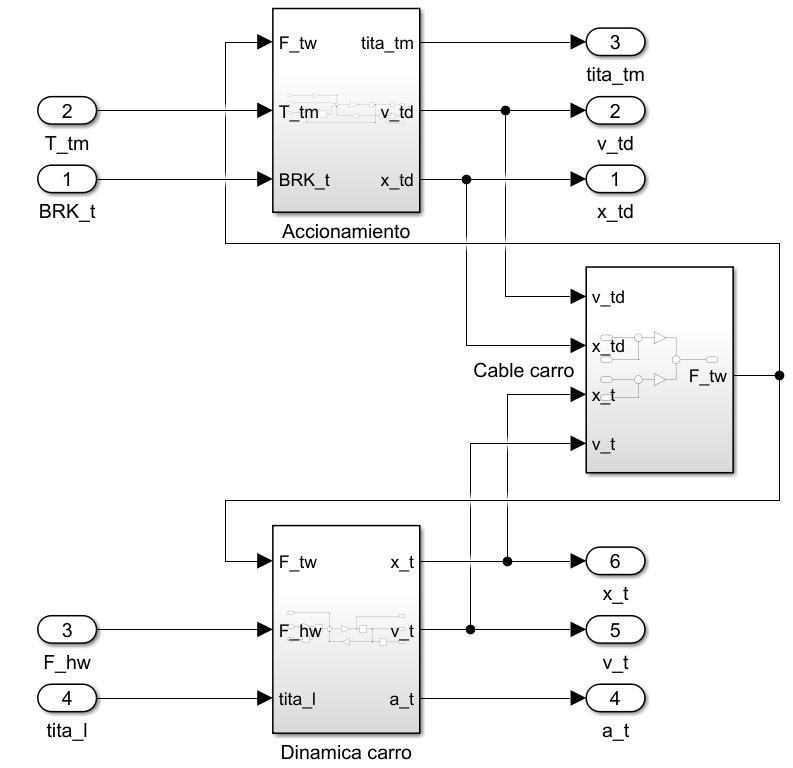
\includegraphics[width=\linewidth]{modelo_carro.png}
    \end{column}
  \end{columns}

  % \vspace{-0.2cm}
  \begin{alertblock}{Dimensionalidad}
    \textbf{3 estados continuos} ($\omega_{tm}, v_t, x_t$) + el \textbf{freno} como evento discreto
    (\sig{$BRK_t$}).
  \end{alertblock}
\end{frame}
